\begin{enumerate}[label=\thechapter.\arabic*,ref=\thechapter.\theenumi]
\item Find the sum of the first $15$ multiples of $8$. \\

\solution
\iffalse
\let\negmedspace\undefined
\let\negthickspace\undefined
\documentclass[journal,12pt,twocolumn]{IEEEtran}
\usepackage{cite}
\usepackage{amsmath,amssymb,amsfonts,amsthm}
\usepackage{algorithmic}
\usepackage{graphicx}
\usepackage{textcomp}
\usepackage{xcolor}
\usepackage{txfonts}
\usepackage{listings}
\usepackage{enumitem}
\usepackage{mathtools}
\usepackage{gensymb}
\usepackage{comment}
\usepackage[breaklinks=true]{hyperref}
\usepackage{tkz-euclide} 
\usepackage{listings}
\usepackage{gvv}                                        
\def\inputGnumericTable{}                                 
\usepackage[latin1]{inputenc}                                
\usepackage{color}                                            
\usepackage{array}                                            
\usepackage{longtable}                                       
\usepackage{calc}                                             
\usepackage{multirow}                                         
\usepackage{hhline}                                           
\usepackage{ifthen}                                           
\usepackage{lscape}
\newtheorem{theorem}{Theorem}[section]
\newtheorem{problem}{Problem}
\newtheorem{proposition}{Proposition}[section]
\newtheorem{lemma}{Lemma}[section]
\newtheorem{corollary}[theorem]{Corollary}
\newtheorem{example}{Example}[section]
\newtheorem{definition}[problem]{Definition}
\newcommand{\BEQA}{\begin{eqnarray}}
\newcommand{\EEQA}{\end{eqnarray}}
\newcommand{\define}{\stackrel{\triangle}{=}}
\theoremstyle{remark}

\newtheorem{rem}{Remark}
\begin{document}
\parindent 0px
\bibliographystyle{IEEEtran}
\title{Assignment 10.5.3\_13Q}
\author{EE23BTECH11219 - Rada Sai Sujan$^{}$% <-this % stops a space
}
\maketitle
\newpage
\bigskip
\section*{Question}
Find the sum of the first $15$ multiples of $8$. \\
\solution
\fi

\begin{table}[ht]
    \centering
    \def\arraystretch{1.5}
    \begin{tabular}{|p{2cm}|p{2.5cm}|p{2.3cm}|}
    \hline
    PARAMETER & VALUE & DESCRIPTION  \\ \hline
    $$x\brak0$$ & $$8$$ & First term \\ \hline
    $$d$$ & $$8$$ & common difference \\ \hline
    $$x(n)$$ & $$[8+8n]u\brak n$$ & General term of the series  \\ 
    \hline
  \end{tabular}

    \caption{Parameter Table1}
    \label{tab:10.5.3.1}
\end{table}
For an $AP$,
\begin{align}
    X\brak z &= \frac{ x\brak 0 }{1-z^{-1}} + \frac{dz^{-1}}{{(1-z^{-1})}^{2}}    \\
    \implies X\brak z &= \frac{8}{1-z^{-1}} + \frac{8z^{-1}}{{(1-z^{-1})}^{2}} \\
    &= \frac{8}{({1-z^{-1})}^{2}} ,\quad \abs{z}>1    \\
    y\brak{n}&=x\brak{n}\ast u\brak{n}\\
    \implies Y\brak{z}&=X\brak{z}U\brak{z}   \\
    Y\brak{z}&=\brak{\frac{8}{({1-z^{-1})}^{2}}}\brak{\frac{1}{1-z^{-1}}}  \\
    &=\frac{8}{({1-z^{-1})}^{3}} ,\quad \abs{z}>1 
\end{align}
 Using Contour Integration to find the inverse $Z$-transform,
\begin{align}
    y(14)&=\frac{1}{2\pi j}\oint_{C}Y(z) \;z^{13} \;dz  \\
    &=\frac{1}{2\pi j}\oint_{C}\frac{8z^{13}}{({1-z^{-1})}^{3}} \;dz 
\end{align}
We can observe that the pole is repeated $3$ times and thus $m=3$,
\begin{align}
    R&=\frac{1}{\brak {m-1}!}\lim\limits_{z\to a}\frac{d^{m-1}}{dz^{m-1}}\brak {{(z-a)}^{m}f\brak z}  \\
    &=\frac{1}{\brak {2}!}\lim\limits_{z\to 1}\frac{d^{2}}{dz^{2}}\brak {{(z-1)}^{3}\frac{8z^{16}}{{(z-1)}^3}}   \\
    &=4\lim\limits_{z\to 1}\frac{d^2}{dz^2}(z^{16})   \\
    &=960
\end{align}
\begin{align}
    \therefore \boxed{y(14)=960}
\end{align}
\begin{figure}[ht]
        \centering
        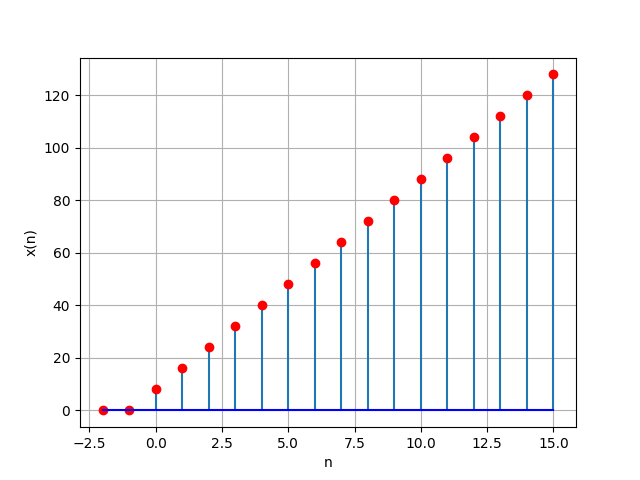
\includegraphics[width=\columnwidth]{ncert-maths/10/5/3/13/figs/a.png}
        \caption{Plot of x(n) $vs$ n}
        \label{fig:10.5.3.13.1}
    \end{figure}
    

%\pagebreak

\item If the sum of $n$ terms of an A.P. is $3n^2+5n$ and its $m^{th}$ term is 164, find the value of $m$.\\
\solution
\iffalse
\documentclass[journal,12pt,twocolumn]{IEEEtran}
\usepackage{amsmath,amssymb,amsfonts,amsthm}
\usepackage{txfonts}
\usepackage{tkz-euclide}
\usepackage{listings}
\usepackage{gvv}
\usepackage[latin1]{inputenc}
\usepackage{array}
\usepackage{pgf}
\usepackage{lmodern}

\begin{document}
\bibliographystyle{IEEEtran}

\vspace{3cm}

\title{}
\author{EE23BTECH11054 -  Sai Krishna Shanigarapu$^{*}$
}
\maketitle
\newpage
\bigskip



\section*{Exercise 9.2}

13. \hspace{2pt}If the sum of $n$ terms of an A.P. is $3n^2+5n$ and its $m^{th}$ term is 164, find the value of $m$.
\bigskip

\solution
\fi
\begin{align}
Y\brak{z} &=  \sum_{n=0}^{\infty} y\brak{n}z^{-n} \\
&= \frac{2\brak{4-z^{-1}}}{\brak{1-z^{-1}}^3}, \qquad |z| > 1\\
U\brak{z} &= \frac{1}{1-z^{-1}}, \qquad |z| > 1\\
X\brak{z} &=  \frac{Y\brak{z}}{U\brak{z}}\\
 &= 2\brak{\frac{1}{1-z^{-1}}} + 6\brak{\frac{1}{\brak{1-z^{-1}}^2} } \\
 &= \frac{8z^2 - 2z}{\brak{z-1}^2} 
\end{align}


Using Contour Integration to find the inverse Z-transform,
\begin{align}
   x\brak{n} &= \frac{1}{2\pi j}\oint_C X\brak{z}z^{n-1}dz\\
    &= \frac{1}{2\pi j}\oint_C \frac{\brak{8z^{n+1} - 2z^{n}}dz}{\brak{z-1}^2}\\
    &= \frac{1}{\brak{m-1}!}\lim_{z\to\ a}\frac{d^{m-1}}{dz^{m-1}}\brak{\brak{z-a}^m f\brak{z}}\\
    &= \lim_{z\to\ 1}\frac{d}{dz}\brak{\brak{z-1}^2 \frac{8z^{n+1} - 2z^n}{\brak{z-1}^2}}\\
    &= \lim_{z\to 1}\brak{8\brak{n+1}z^n - 2nz^{n-1}}\\
    \implies x\brak{n} &= \brak{6n+8}\brak{u\brak{n}}\\
    164 &= \brak{6m+8}\brak{u\brak{m}}\\
    \implies m &= 26
\end{align}

\setlength{\arrayrulewidth}{0.3mm}
\setlength{\tabcolsep}{15pt}
\renewcommand{\arraystretch}{1.4}

\begin{table}[ht]
\centering

\begin{tabular}{|c|c|}
\hline

Symbol & Remarks\\
\hline
$y\brak{n} =\brak{3n^2+11n+8}\brak{u\brak{n}}$ & Sum of $n$ terms  \\
\hline
$x(m-1)$ & $164$\\
\hline
$y\brak{n}$ & $x\brak{n} * u\brak{n}$\\
\hline

\end{tabular}
\vspace{0.25cm}
\caption{Parameters}
\label{tab:11.9.2.13.1}



\end{table}



\begin{figure}[htbp]
    \centering
    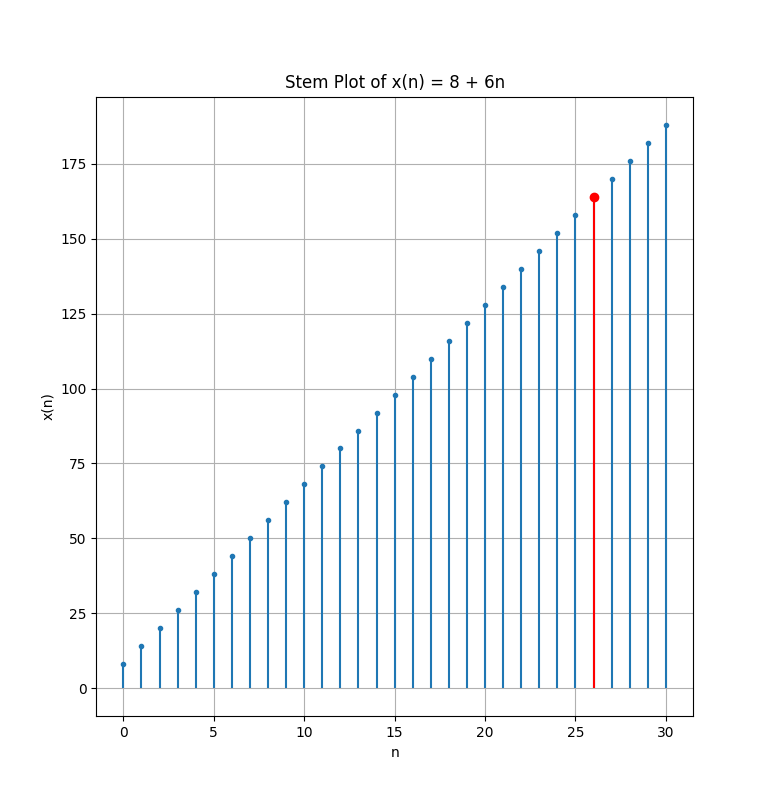
\includegraphics[width=1.0\columnwidth]{ncert-maths/11/9/2/13/figs/Figure_1.png}
    \caption{Plot of x(n) vs n}
    \label{fig:11.9.2.13.1}
\end{figure}


%\end{document}


\pagebreak
\item Show that $a_0$ , $a_1$ , $a_2$
, . . ., $a_n$
, . . . form an AP where an is defined as below :
\begin{enumerate}
    \item $a_n$ = $(3 + 4n)$ 
    \item $a_n$ = $(9 - 5n)$ 
\end{enumerate}
Also find the sum of the first 15 terms in each case.
\solution
\iffalse
\let\negmedspace\undefined
\let\negthickspace\undefined
\documentclass[journal,12pt,twocolumn]{IEEEtran}
\usepackage{cite}
\usepackage{amsmath,amssymb,amsfonts,amsthm}
\usepackage{algorithmic}
\usepackage{graphicx}
\usepackage{textcomp}
\usepackage{xcolor}
\usepackage{txfonts}
\usepackage{listings}
\usepackage{enumitem}
\usepackage{mathtools}
\usepackage{gensymb}
\usepackage{comment}
\usepackage[breaklinks=true]{hyperref}
\usepackage{tkz-euclide} 
\usepackage{listings}
\usepackage{gvv}                                        
\def\inputGnumericTable{}                                 
\usepackage[latin1]{inputenc}                                
\usepackage{color}                                            
\usepackage{array}                                            
\usepackage{longtable}                                       
\usepackage{calc}                                             
\usepackage{multirow}                                         
\usepackage{hhline}                                           
\usepackage{ifthen}                                           
\usepackage{lscape}
\usepackage{amsmath}
\usepackage{caption}
\newtheorem{theorem}{Theorem}[section]
\newtheorem{problem}{Problem}
\newtheorem{proposition}{Proposition}[section]
\newtheorem{lemma}{Lemma}[section]
\newtheorem{corollary}[theorem]{Corollary}
\newtheorem{example}{Example}[section]
\newtheorem{definition}[problem]{Definition}
\newcommand{\BEQA}{\begin{eqnarray}}
\newcommand{\EEQA}{\end{eqnarray}}
\newcommand{\define}{\stackrel{\triangle}{=}}
\theoremstyle{remark}
\newtheorem{rem}{Remark}
\begin{document}

\bibliographystyle{IEEEtran}
\vspace{3cm}

\title{NCERT 10.5.3 10Q}
\author{EE22BTECH11010 - Venkatesh D Bandawar $^{*}$% <-this % stops a space
}
\maketitle
\newpage
\bigskip

\renewcommand{\thefigure}{\theenumi}
\renewcommand{\thetable}{\theenumi}

\textbf{Question:} Show that $a_0$ , $a_1$ , $a_2$
, . . ., $a_n$
, . . . form an AP where an is defined as below :
\begin{enumerate}
    \item $a_n$ = $(3 + 4n)$ 
    \item $a_n$ = $(9 - 5n)$ 
\end{enumerate}
Also find the sum of the first 15 terms in each case.

\textbf{Solution:} 
\fi
    \begin{table}[!h] 
    \centering
    \begin{tabular}{|c|c|c|}
\hline
     \textbf{Parameter} & \textbf{Description} & \textbf{Value} \\
     \hline
     \multirow{3}{*}{$x_i(n)$} & \multirow{3}{*}{$i^{th}$Discrete signal} & $(3+4n)u(n)$\\
     \cline{3-3}
     & & $(9-5n)u(n)$\\
     \hline
     \multirow{3}{*}{$x_i(0)$} & \multirow{3}{*}{First term of $i^{th}$AP} & $3$ \\
     \cline{3-3}
     & & $9$\\
     \hline
     \multirow{3}{*}{$d_i$} & \multirow{3}{*}{common difference of $i^{th}$AP} & $4$ \\
     \cline{3-3}
     & & $-5$\\
     \hline
\end{tabular}

    \caption{Given parameters}
    \label{given parameters list}
    \end{table}
\begin{enumerate} 
    \item From equation \eqref{eq:APSum}
    \begin{align}
        X(z) &= \frac{3}{1-z^{-1}} + \frac{4.z^{-1}}{(1-z^{-1})^2} ; |z|>1\\
        \because y(n) &= x(n) * u(n)\\
        Y(z) &= X(z)U(z)\\
        &= \sbrak{\frac{3}{\brak{1-z^{-1}}^2} + \frac{4 z^{-1}}{\brak{1-z^{-1}}^3}} 
    \end{align}
    Using contour integration for inverse Z transformation,
    \begin{align}
        y(14) &= \frac{1}{2\pi j}\int Y(z) z^{13} dz \\
         &= \frac{1}{2\pi j}\int \frac{3.z^{15}}{(z-1)^{2}} dz + \frac{1}{2\pi j}\int \frac{4.z^{15}}{(z-1)^{3}} dz\\
        \because R&=\frac{1}{\brak {m-1}!}\lim\limits_{z\to a}\frac{d^{m-1}}{dz^{m-1}}\brak {{(z-a)}^{m}f\brak z}\\
        R_1 &=\frac{1}{1!}\lim\limits_{z\to 1}\frac{d}{dz}\brak {(z-1)^2.\frac{3.z^{15}}{(z-1)^{2}}}\\
        &= 45\\
        R_2 &=\frac{1}{2!}\lim\limits_{z\to 1}\frac{d^2}{dz^2}\brak {(z-1)^3.\frac{4.z^{15}}{(z-1)^{3}}}\\
        &= 420\\
        \implies y(14) &= R_1 + R_2 \\
        &= 465
    \end{align}
    
    \begin{figure}[!h] 
    \centering
    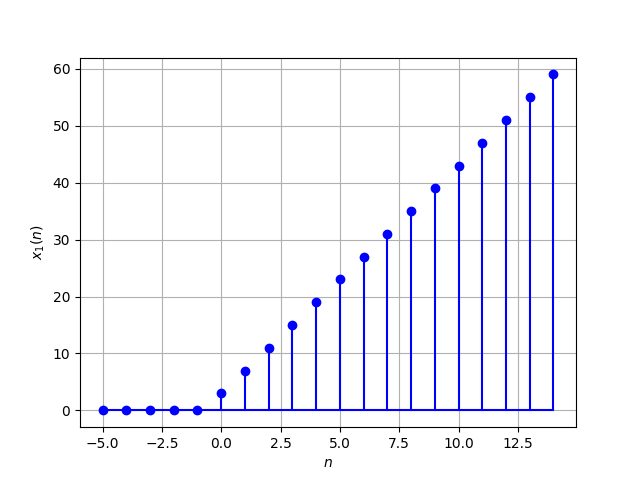
\includegraphics[width=\columnwidth]{ncert-maths/10/5/3/10/figs/signal_x1.png}
    \caption{$x_1(n)=(3+4n)u(n)$}
    \label{fig:Graph1_math.10.5.3.10}
    \end{figure}

    \begin{figure}[!h] 
    \centering
    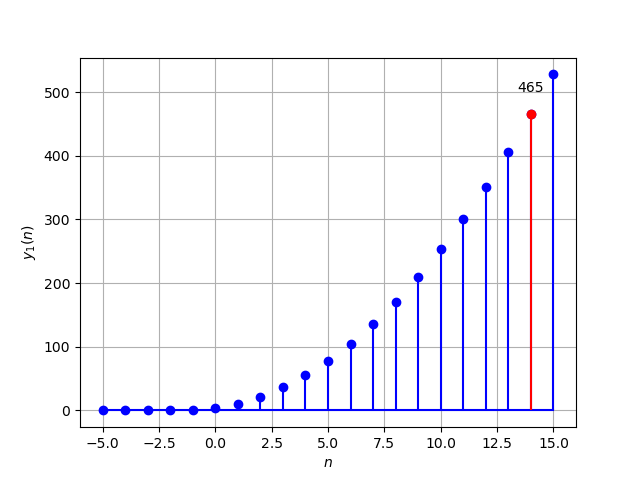
\includegraphics[width=\columnwidth]{ncert-maths/10/5/3/10/figs/signal_y1.png}
    \caption{$x_1(n)=(2n^2+5n+3)u(n)$}
    \label{fig:Graph2_math.10.5.3.10}
    \end{figure}
    
    \item From equation  \eqref{eq:APSum}
    \begin{align}
         X(z) &= \frac{9}{1-z^{-1}} - \frac{5.z^{-1}}{(1-z^{-1})^2} ; |z|>1\\
        \because y(n) &= x(n) * u(n)\\
        Y(z) &= X(z)U(z)\\
         &= \sbrak{\frac{9}{\brak{1-z^{-1}}^2} - \frac{5 z^{-1}}{\brak{1-z^{-1}}^3}}
    \end{align}
    Using contour integration for inverse Z transformation,
    \begin{align}
       y(14) &= \frac{1}{2\pi j}\int Y(z) z^{13} dz \\
         &= \frac{1}{2\pi j}\int \frac{9.z^{15}}{(z-1)^{2}} dz - \frac{1}{2\pi j}\int \frac{5.z^{15}}{(z-1)^{3}} dz\\
        \because R&=\frac{1}{\brak {m-1}!}\lim\limits_{z\to a}\frac{d^{m-1}}{dz^{m-1}}\brak {{(z-a)}^{m}f\brak z}\\
        R_1 &=\frac{1}{1!}\lim\limits_{z\to 1}\frac{d}{dz}\brak {(z-1)^2.\frac{9.z^{15}}{(z-1)^{2}}}\\
         &= 135\\
        R_2 &=\frac{1}{2!}\lim\limits_{z\to 1}\frac{d^2}{dz^2}\brak {(z-1)^3.\frac{5.z^{15}}{(z-1)^{3}}}\\
         &= 525\\
        \implies y(14) &= R_1 - R_2 \\
        &= -390
    \end{align}
    
    \begin{figure}[!h] 
    \centering
    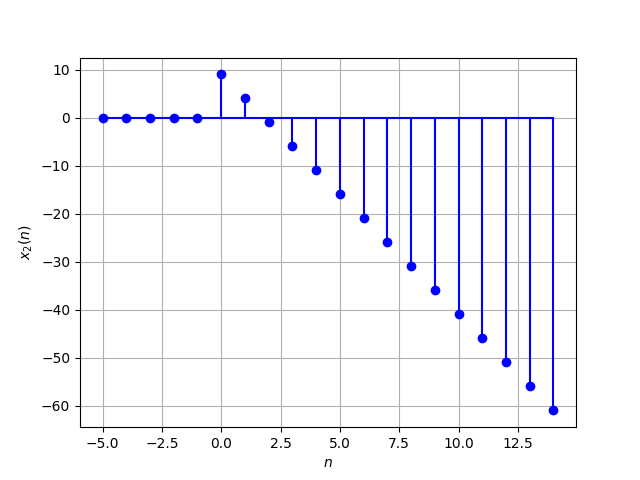
\includegraphics[width=\columnwidth]{ncert-maths/10/5/3/10/figs/signal_x2.png}
    \caption{$x_2(n)=(9-5n)u(n)$}
    \label{fig:Graph3_math.10.5.3.10}
    \end{figure}

    \begin{figure}[!h] 
    \centering
    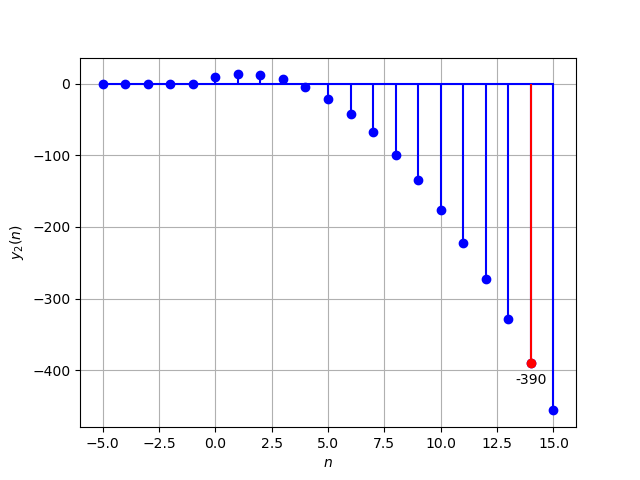
\includegraphics[width=\columnwidth]{ncert-maths/10/5/3/10/figs/signal_y2.png}
    \caption{$x_2(n)=(-5n^2+13n+18)u(n)$}
    \label{fig:Graph4_math.10.5.3.10}
    \end{figure}

\end{enumerate} 


\pagebreak
\item If the sum of $n$ terms of an AP is $(pn + qn^2)$, where $p$ and $q$ are constants, find the common difference.
\solution
		\iffalse
\let\negmedspace\undefined
\let\negthickspace\undefined
\documentclass[journal,12pt,twocolumn]{IEEEtran}
\usepackage{cite}
\usepackage{amsmath,amssymb,amsfonts,amsthm}
\usepackage{algorithmic}
\usepackage{graphicx}
\usepackage{textcomp}
\usepackage{xcolor}
\usepackage{txfonts}
\usepackage{listings}
\usepackage{enumitem}
\usepackage{mathtools}
\usepackage{gensymb}
\usepackage{comment}
\usepackage[breaklinks=true]{hyperref}
\usepackage{tkz-euclide} 
\usepackage{listings}
\usepackage{gvv}                                        
\def\inputGnumericTable{}                                
\usepackage[latin1]{inputenc}                            
\usepackage{color}                                       
\usepackage{array}                                       
\usepackage{longtable}                                   
\usepackage{calc}                              
\usepackage{tikz}
\usepackage{multirow}                                    
\usepackage{hhline}                                      
\usepackage{ifthen}                            
\usepackage{caption}
\usepackage{lscape}
\usepackage{amsmath}
\newtheorem{theorem}{Theorem}[section]
\newtheorem{problem}{Problem}
\newtheorem{proposition}{Proposition}[section]
\newtheorem{lemma}{Lemma}[section]
\newtheorem{corollary}[theorem]{Corollary}
\newtheorem{example}{Example}[section]
\newtheorem{definition}[problem]{Definition}
\newcommand{\BEQA}{\begin{eqnarray}}
\newcommand{\EEQA}{\end{eqnarray}}
\newcommand{\define}{\stackrel{\triangle}{=}}
\theoremstyle{remark}
\newtheorem{rem}{Remark}

\begin{document}

\bibliographystyle{IEEEtran}
\vspace{3cm}

\title{NCERT Math 11.9.2 Q8}
\author{EE23BTECH11009 - AROSHISH PRADHAN$^{*}$% <-this % stops a space
}
\maketitle
\newpage
\bigskip
\textbf{Question:} If the sum of $n$ terms of an AP is $(pn + qn^2)$, where $p$ and $q$ are constants, find the common difference.

\solution
\fi
\begin{table}[!h]
    \centering
    \begin{tabular}{|c|c|c|}
    \hline
      \textbf{Symbol}   &  \textbf{Value} & \textbf{Description}\\
    \hline
       $y(n)$  & $(pn + qn^2)$ & Sum of $n$ terms\\
    \hline
        $x(n)$ &  & $n^{th}$ term of AP\\
    \hline
        $d$ & $x(n+1) - x(n)$ &Common Difference\\
    \hline 
\end{tabular}

    \caption{Given Parameters}
    \label{tab:1_Math.11.9.2.8}
\end{table}

Sum of $n$ terms, as a discrete signal:
\begin{align}
    y(n) = (pn + qn^2)u(n) \label{eq:1_Math.11.9.2.8}
\end{align}
Taking the $Z$-Transform,
\begin{enumerate}
    \item $\mathcal{Z}\{u(n)\}$
\begin{align}
    u(n) \system{Z} \frac{1}{1-z^{-1}} \{\abs{z} > 1\} \label{eq:2_Math.11.9.2.8}
\end{align}
    \item $\mathcal{Z}\{nu(n)\}$
\begin{align}
    nu(n) \system{Z} \frac{z^{-1}}{(1-z^{-1})^2}\, \{\abs{z} > 1\} \label{eq:3_Math.11.9.2.8}
\end{align}
\item $\mathcal{Z}{\{n^2 u(n)\}}$
    \begin{align}
        n^2u(n) \system{Z} \frac{z^{-1}(1+z^{-1})}{(1-z^{-1})^3}\, \{\abs{z} > 1\} \label{eq:4_Math.11.9.2.8}
    \end{align}
\end{enumerate}
Taking the Z-Transform of \eqref{eq:1_Math.11.9.2.8} using \eqref{eq:3_Math.11.9.2.8} and \eqref{eq:4_Math.11.9.2.8}
\begin{align}
      Y(z) = p\brak{\frac{z^{-1}}{(1-z^{-1})^2}} + q\brak{\frac{z^{-1}(1 + z^{-1})}{(1-z^{-1})^3}}
\end{align}
Now, 
\begin{align}
    y(n) &= x(n) \ast u(n)\\
    \implies Y(z) &= X(z)U(z)\\
    \implies X(z) &= \frac{Y(z)}{U(z)}\label{eq:8_Math.11.9.2.8}
\end{align}
Using \eqref{eq:2_Math.11.9.2.8} in \eqref{eq:8_Math.11.9.2.8},
\begin{align}
    X(z) &= p\brak{\frac{z^{-1}}{(1-z^{-1})}} + q\brak{\frac{z^{-1}(1 + z^{-1})}{(1-z^{-1})^2}}
\end{align}
Using contour integration for inverse Z-Transform:
\begin{align}
    x(n) &= \frac{1}{2\pi j} \oint_C X(z) z^{n-1}dz\\
    &= \frac{1}{2 \pi j} \oint_C  \sbrak{p\brak{\frac{z^{-1}}{(1-z^{-1})}} + q\brak{\frac{z^{-1}(1 + z^{-1})}{(1-z^{-1})^2}}}z^{n-1}dz
\end{align}
Calculating the residues $R_1$ and $R_2$ at pole $z=1$:
\begin{align}
    R_1 &= \frac{1}{0!} \lim_{z \to 1}(z-1)\brak{p\brak{\frac{z^{-1}}{1-z^{-1}}}}z^{n-1}\\
    &= p\\
    R_2 &= \frac{1}{1!} \lim_{z \to 1}\frac{d}{dz}\brak{(z-1)^2q\brak{\frac{z^{-1}(1 + z^{-1})}{(1-z^{-1})^2}}}z^{n-1}\\
    &= q\lim_{z \to 1}\frac{d}{dz}\brak{z^{n} + z^{n-1}}\\
    &= q(2n-1)\\
    \implies x(n) &= R_1 + R_2\\
    &= p + q(2n-1)
\end{align}
Writing x(n) as a discrete signal we get:
\begin{align}
    x(n) &= (p-q)u(n) + 2qnu(n)\label{eq:19_Math.11.9.2.8}
\end{align}
To simplify, use $n=0$:
\begin{align}
    y(0)&=x(0)\\
    \implies 0 &= (p-q)u(0) +2q(0)u(0)\\
    \implies p &= q
\end{align}
$\therefore$ \eqref{eq:19_Math.11.9.2.8} an be written as:
\begin{align}
    x(n) &= 2qnu(n)
\end{align}
Common difference is given by:
\begin{align}
    d &= x(n+1) - x(n)\\
    &= 2q
\end{align}
\begin{figure}[!h]
    \centering
    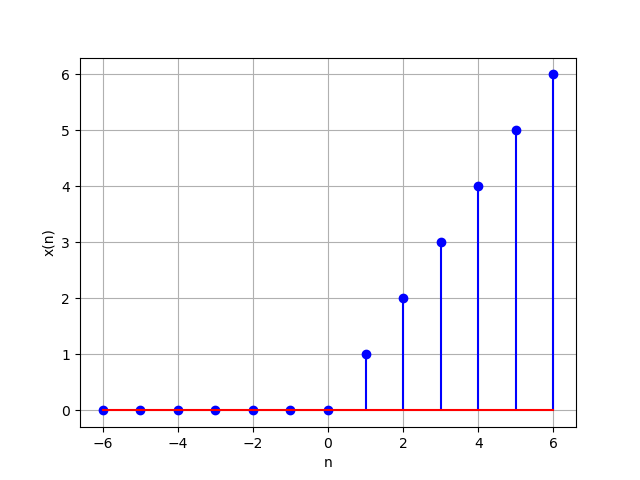
\includegraphics[width = \columnwidth]{ncert-maths/11/9/2/8/figs/x_plot.png}
    \caption{Plot of x(n) vs n for $p=q=0.5$}
    \label{fig:1_Math.11.9.2.8}
\end{figure}
\begin{figure}[!h]
    \centering
    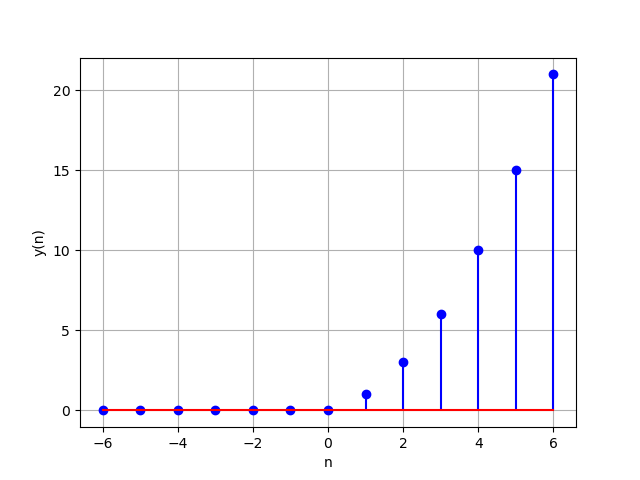
\includegraphics[width = \columnwidth]{ncert-maths/11/9/2/8/figs/y_plot.png}
    \caption{Plot of y(n) vs n for $p=q=0.5$}
    \label{fig:2_Math.11.9.2.8}
\end{figure}

\end{enumerate}
